\section{Problem Definition}
\label{sec:problemdef}
In this section, we define the terminologies used in the paper and give a formal definition of the problem under consideration.

\begin{definition} [Probabilistic link travel times]
In a road network, for every link $(i, j)$ we define the probabilistic link travel time of link $(i,j)$, $c_{ij}^t(x)$, as the probability of taking $x$ seconds for a vehicle to traverse link $(i,j)$ starting at time $t$.
\end{definition}

The link travel times are thus time dependent and differ depending on the arrival time of the vehicle at that starting point of the link. Additionally we consider $c_{ij}^t$ to be a random variable with $f_{ij}^t$ representing its \textit{pdf}.

\begin{definition} [Route pdf (\textbackslash pmf)]
Assuming $p_{sd}$ represents a path starting from point $s$ and ending in point $d$, we define $\pi_{sd}^t$ as the random variable representing the travel time on $p_{sd}$ when we start at time $t$. Accordingly, the route pdf, $J_{sd}^t(x)$, gives the probability of taking $x$ seconds for a vehicle to traverse $p_{sd}$ starting at time $t$.
\end{definition}

The problem considered in this paper is how to  accurately estimate $c_{ij}^t$.

%Consider a directed and connected transportation network $G(V, E, S)$ consisting of a set of nodes $V$, a set of links $E$ and a probability distribution $S$ describing the statistics of the link travel times. The link travel time $c_{ij}^t$ of an edge  $(i,j) ((i,j) \in E, i, j \in V)$ defines the time it takes for a vehicle to traverse the edge when starting at time $t$ at node $i$. The link travel times are thus time dependent and differ depending on the arrival time of the vehicle at that edge. Additionally we consider $c_{ij}^t$ to be a random variable with $f_{ij}^t$ representing its \textit{pdf}. The problem considered in this paper is how to obtain the \textit{pdf} for $c_{ij}^t$. Later on, such \textit{pdf} is used to build a \textit{pdf} for an entire route. If $p_{sd}$ represents a path from node $s$ to node $d$ we call $\pi_{sd}$ the random variable representing the travel time on $p_{sd}$. 

%Existing studies so far focused on different algorithms combining given \textit{pltts} and forming a \textit{pdf} for the entire route. However, to the best of our knowledge none of these studies have considered generating the \textit{pltts} themselves. Hence, none of these studies are able to examine the whole pipeline from the raw real-data to the probabilistic outcome and evaluate them properly - which poses several additional challenges. Towards this end, in addition to proposing techniques to generate \textit{pltts}, we also see this work as a study on how to evaluate probabilistic approaches on uncertain data in a real-wold setting in general. With this paper, we will focus on the following three specific problems:

%\textbf{(1) Probabilistic prediction of edge weights:} We develop techniques that compute probabilistic link travel times. Specifically, we aim at obtaining a \textit{pdf} (or \textit{pmf}) representing $c_{ij}^t$ based on the following data:

%\begin{itemize}
%\item The graph of the road network to consider $G(V,E)$.
%\item For each edge $(i,j) \in E$ historical data about the   link travel time $c_{ij}^t, t \in H = \{-L\phi, (L+1)\phi, \ldots, -\phi\}$, where $\phi$ is the smallest considered time unit and $L \in \NN$.
%\item For each edge $(i,j) \in E$ the current link travel time $c_{ij}^0$.
%\end{itemize}

%\textbf{(2) Technical analysis of existing work:} We classify existing approaches for computing the probabilistic path travel time $\pi^t_{sd}$ according to some of their basic characteristics. Then we apply the different \textit{pltt} generation techniques proposed on this paper to these approaches to evaluate the significance of using a good Vs. bad \textit{pltt} generation technique on the overall outcome.

%\textbf{(3) Evaluation of probabilistic predictions:} The evaluation and comparison of different approaches has to be carried out with a selected repertory from the statistical toolbox. The main challenge here is that the outcome of the methods for a specific starting time $t$ and a path  $p_{sd}$ is a \textit{pdf} over the estimated path travel time $\pi^t_{sd}$. Comparing the outcome with the true travel time over several trials has the challenge that $\pi^t_{sd}$ differs for different starting times. We thus propose a statistical test that enables us to evaluate these outcomes.

% \section{Categorization of Approaches} 
% The above problem statement however is very general and the existing works to
% solve this problem each use a specialized model for $S$. Generally they can be
% categorized by the following three attributes: model for the link travel times,
% consideration of time-dependency and modelling of correlations.
% 
% \subsection{Model for Link Travel Times}
% 
% 
% \subsection{Time Dependency}
% Especially in road-networks time-dependency is a crucial feature which allows
% for a much more precise estimation of the overall travel time. This is obvious
% since the conditions of a road network (including density of vehicles, traffic
% jams, construction sites, accidents) may change rapidly and effect the single
% link travel times drastically. Depending on time $t$ of the day the
% travel time $c_{ij}^t$ for a road segment may thus be represented by a
% different \textit{pdf} (e.g. travel time for the same road segment may be represented either by the \textit{pdf} shown in Figure
% \ref{fig:discrete} for Sundays or by the \textit{pdf} shown in Figure
% \ref{fig:traffic} during rush hours on weekdays).
% 
% \begin{figure}[h]
%     \centering
%     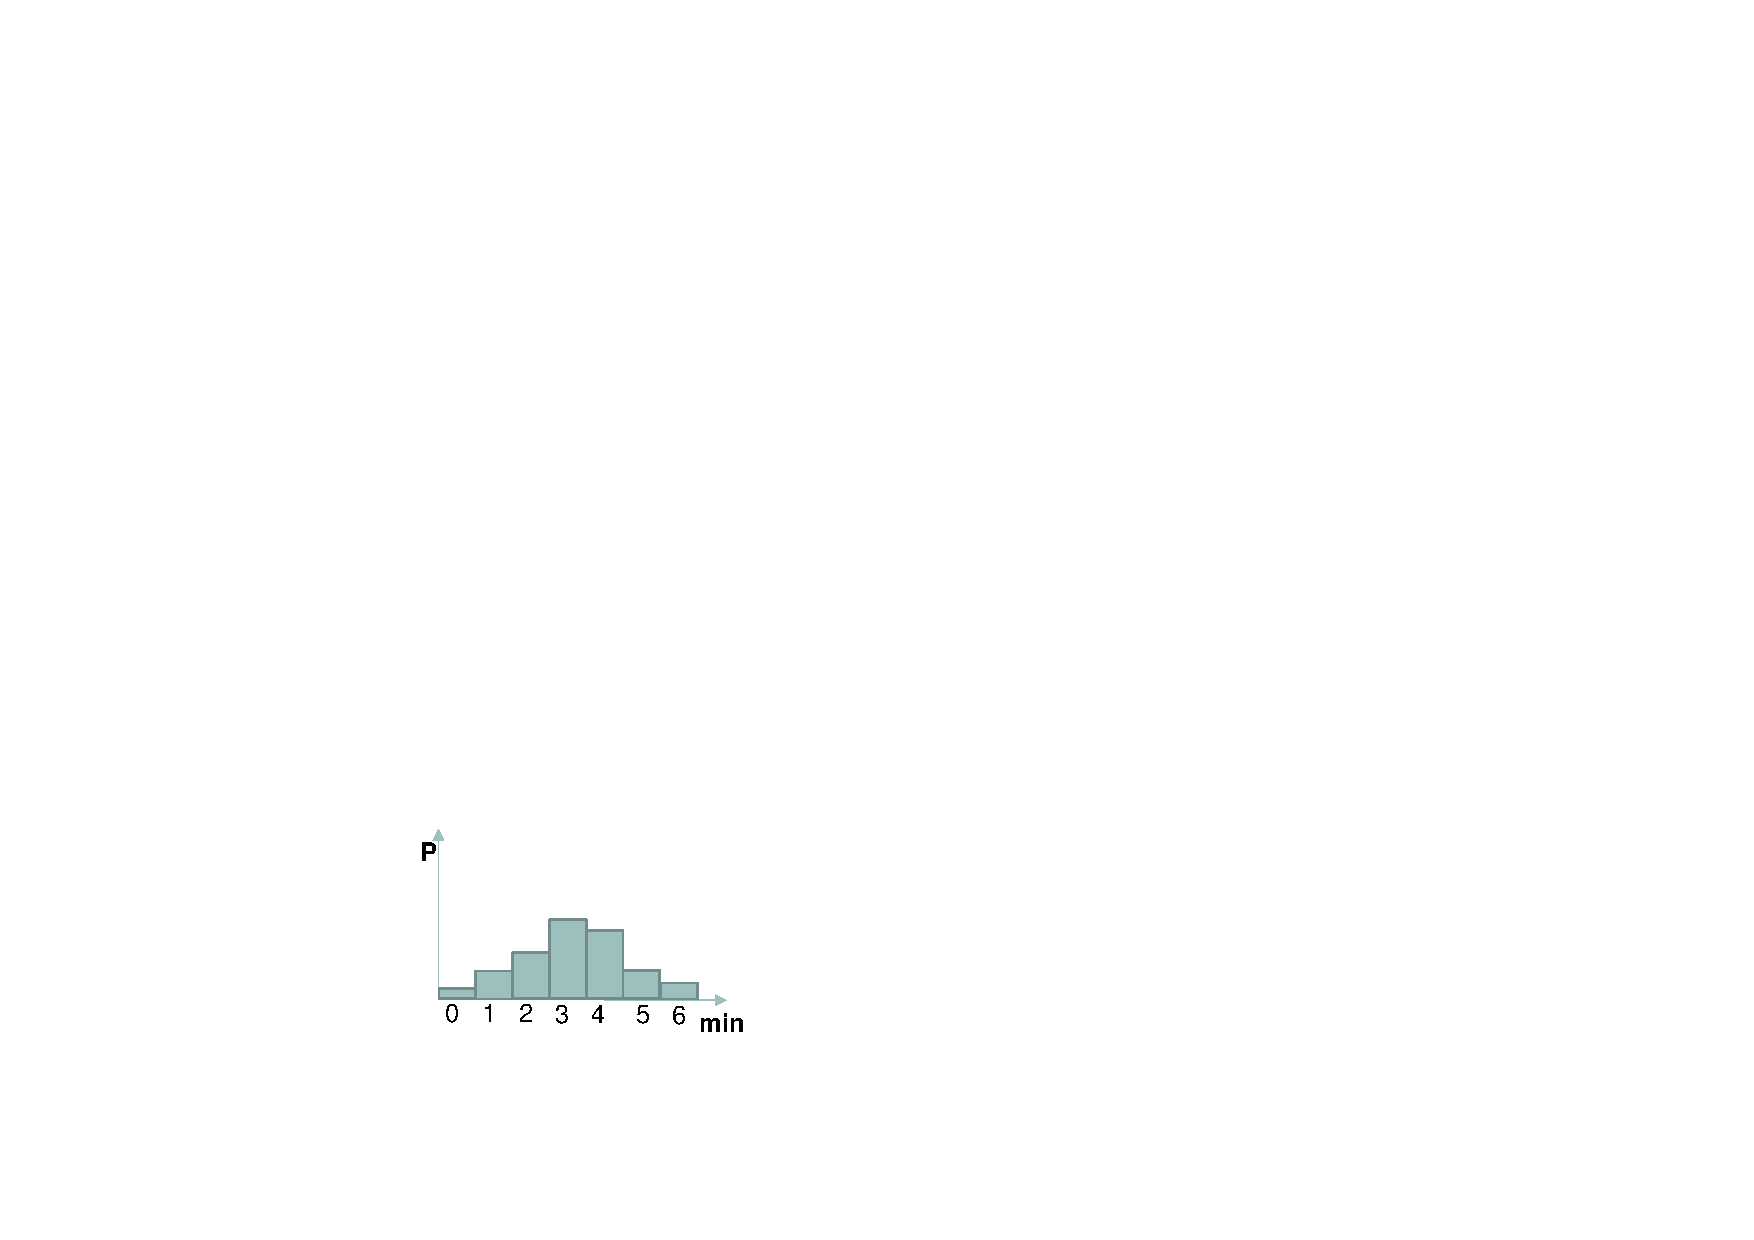
\includegraphics[width=0.5\columnwidth]{figures/pdf_traffic.pdf}
%     \caption{link travel time at rush hour}
%     \label{fig:traffic}
% \end{figure}
% 
% \subsection{Link Travel Time Correlations}
% The last characteristic is the modelling of correlations between link travel
% times. It is possible to treat the link travel times of different road segments
% (edges) as independent random variables. However on a real-world traffic
% network, it might be more realistic to assume correlated link travel times. For
% example if there is a traffic jam on on road segment yielding high travel times
% then it is likely that the subsequent road segment is also jammed and the travel
% time is also high. To model the correlation between random variables, there
% exist several approaches which will be reviewed in the following section.


